We survey the efforts researchers have made to achieve an even better
performance on these three file systems.
%
The better performance here refers to characteristics such as throughput,
scalability, etc.


\subsection{GFS: Toward a Global Scalability}
\label{sec:gfs_scal}
%
\begin{figure}
\centering
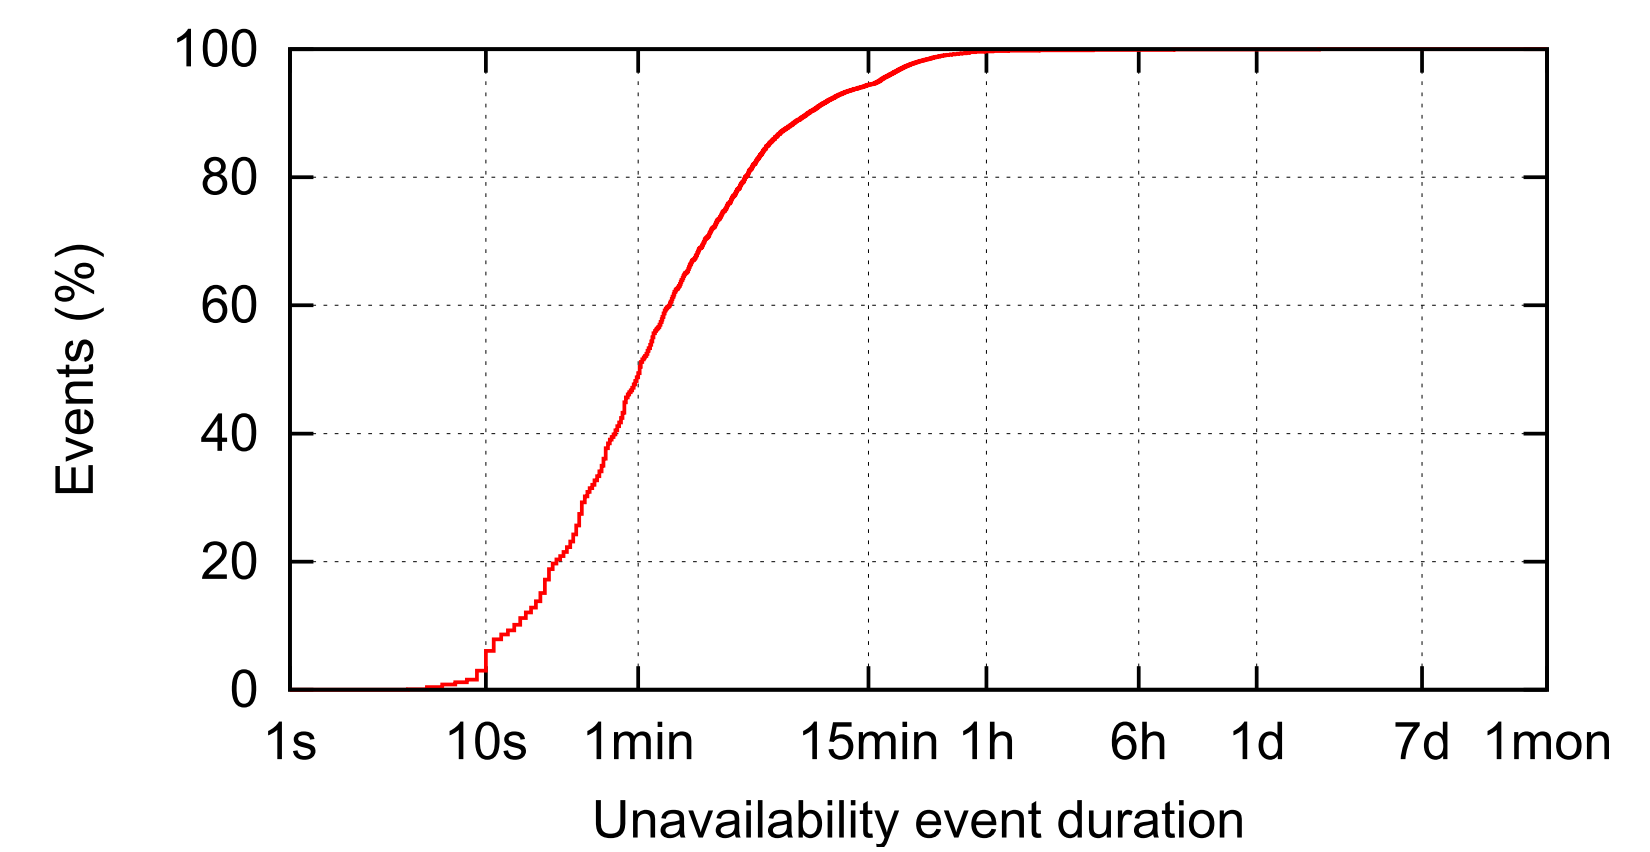
\includegraphics[width=0.99\columnwidth]{image/event.png}
\caption{Cumulative distribution function of the duration of node 
	unavailability periods.}
\label{fig:event}
\end{figure}
%
To achieve great scalability, a good handling of failures is necessary.
%
In the real application of GFS, many storage server nodes are called a cell.
%
A typical cell may comprise many thousands of nodes housed together in a 
single building or a set of co-located buildings.

To characterize the failures and availability of a GFS cell, we start from
the availability of single storage nodes.
%
A storage node becomes unavailable when it fails to respond positively 
to periodic health checking pings.
%
Nodes can become unavailable for a large number of
reasons. For example, a storage node or networking switch can be overloaded; 
a node binary or operating system may crash or restart; 
a machine may experience a hardware error; 
or the whole cluster could be brought down for maintenance. 
%
The vast majority of such unavailability events are transient and do not 
result in permanent data loss.
%
In fact, statistics show that less than 10\% of events last longer than 15 
minutes (see Figure~\ref{fig:event}).
%
For this reason, GFS typically waits 15 minutes before commencing 
recovery of data on unavailable nodes.

Two measurements are used to measure the stability of the GFS: 
average availability and mean time to failure (MTTF). 
%
Given a cluster of $N$ nodes, average availability is defined as following:
%
\begin{equation}
A_{N}=\frac{\sum_{N_i\in N} uptime(N_i)}{\sum_{N_i\in N}(uptime(N_i) + downtime(n_i))}
\end{equation},
%
where $uptime(N_i)$ and $downtime(N_I)$ refer to the length of time a node $N_i$
is available or unavailable.
%
MTTF is defined as following:
\begin{equation}
MTTF=\frac{uptime}{number of failures}.
\end{equation}


\subsubsection{Data Replication and Chunk Placement}
When a node failure causes the unavailability of a chunk within a stripe, 
we initiate a recovery operation for that chunk from the other available 
chunks remaining in the stripe.
%
Distributed file systems will necessarily employ
queues for recovery operations following node failure. 
These queues prioritize reconstruction of stripes which
have lost the most chunks.

To minimize the effect of large failure bursts in a single failure domain,
we also consider a rack-aware policy.
%
A rack-aware policy is one that ensures that no two chunks in a stripe are 
placed on nodes in the same rack.
%
Research has shown that using a rack-aware placement policy increases 
the stripe MTTF by a factor of 3 typically.

The researchers also used a Markov model to validate some findings.
%
Two interesting finds are:
\begin{enumerate}
\item improvements of component failure rates below the node layer
	of the storage stack do not significantly improve data availability.
	For example, a 10\% reduction in the disk failure rate increases 
	stripe availability by less than 1.5\%. On the other hand, cutting node 
	failure rates by 10\% can increase data availability by 18\%. 
\item Replicating data across multiple cells  greatly improves availability 
	because it protects against correlated failures.
	It also greatly increase the inter-cell bandwidth requirement, so there 
	is still trade-offs to make.
\end{enumerate}


\subsubsection{Google Services Built on Top of the GFS}
Because of the extreme scalability of GFS, other services become available
on top of the GFS.
%
Corbett et al.~\cite{Corbett2012a} demonstrated a database system in in Google.
%
It is the first system to distribute data at global scale and support 
externally-consistent distributed transactions. 
%
Chang et al.~\cite{Chang2006a} demonstrated Bigtable, 
a distributed storage system for managing structured data.
%
It is able to scale to a very large size: petabytes of data across thousands of commodity servers.
%
Even though many Google applications place diverse demands on Bigtable, 
Bigtable is still able to provide high-performance solutions for all these
services.



\subsection{GPFS to Achieve Better Performance}
GPFS has demonstrated great performance in high scalability, 
fast scan, and high throughput.
%
There are many research of GPFS on real systems, for example,
Yu et al.~\cite{Yu2006} demonstrated a highly scalable GPFS file system
with satisfactory overall performance;
%
Andrews et al.~\cite{Andrews2005} researched from both theoretical 
and practical sides of the performance of GPFS file system
in an inter-state scale.
%
Further, Freitas et al.~\cite{freitas2011gpfs} reported performance 
of GPFS file system to scan 10 billion files in 43 minutes. 
%
We elaborate these results in the following subsections.

\subsubsection{GPFS to achieve global scalability}
%
\begin{figure}
\centering
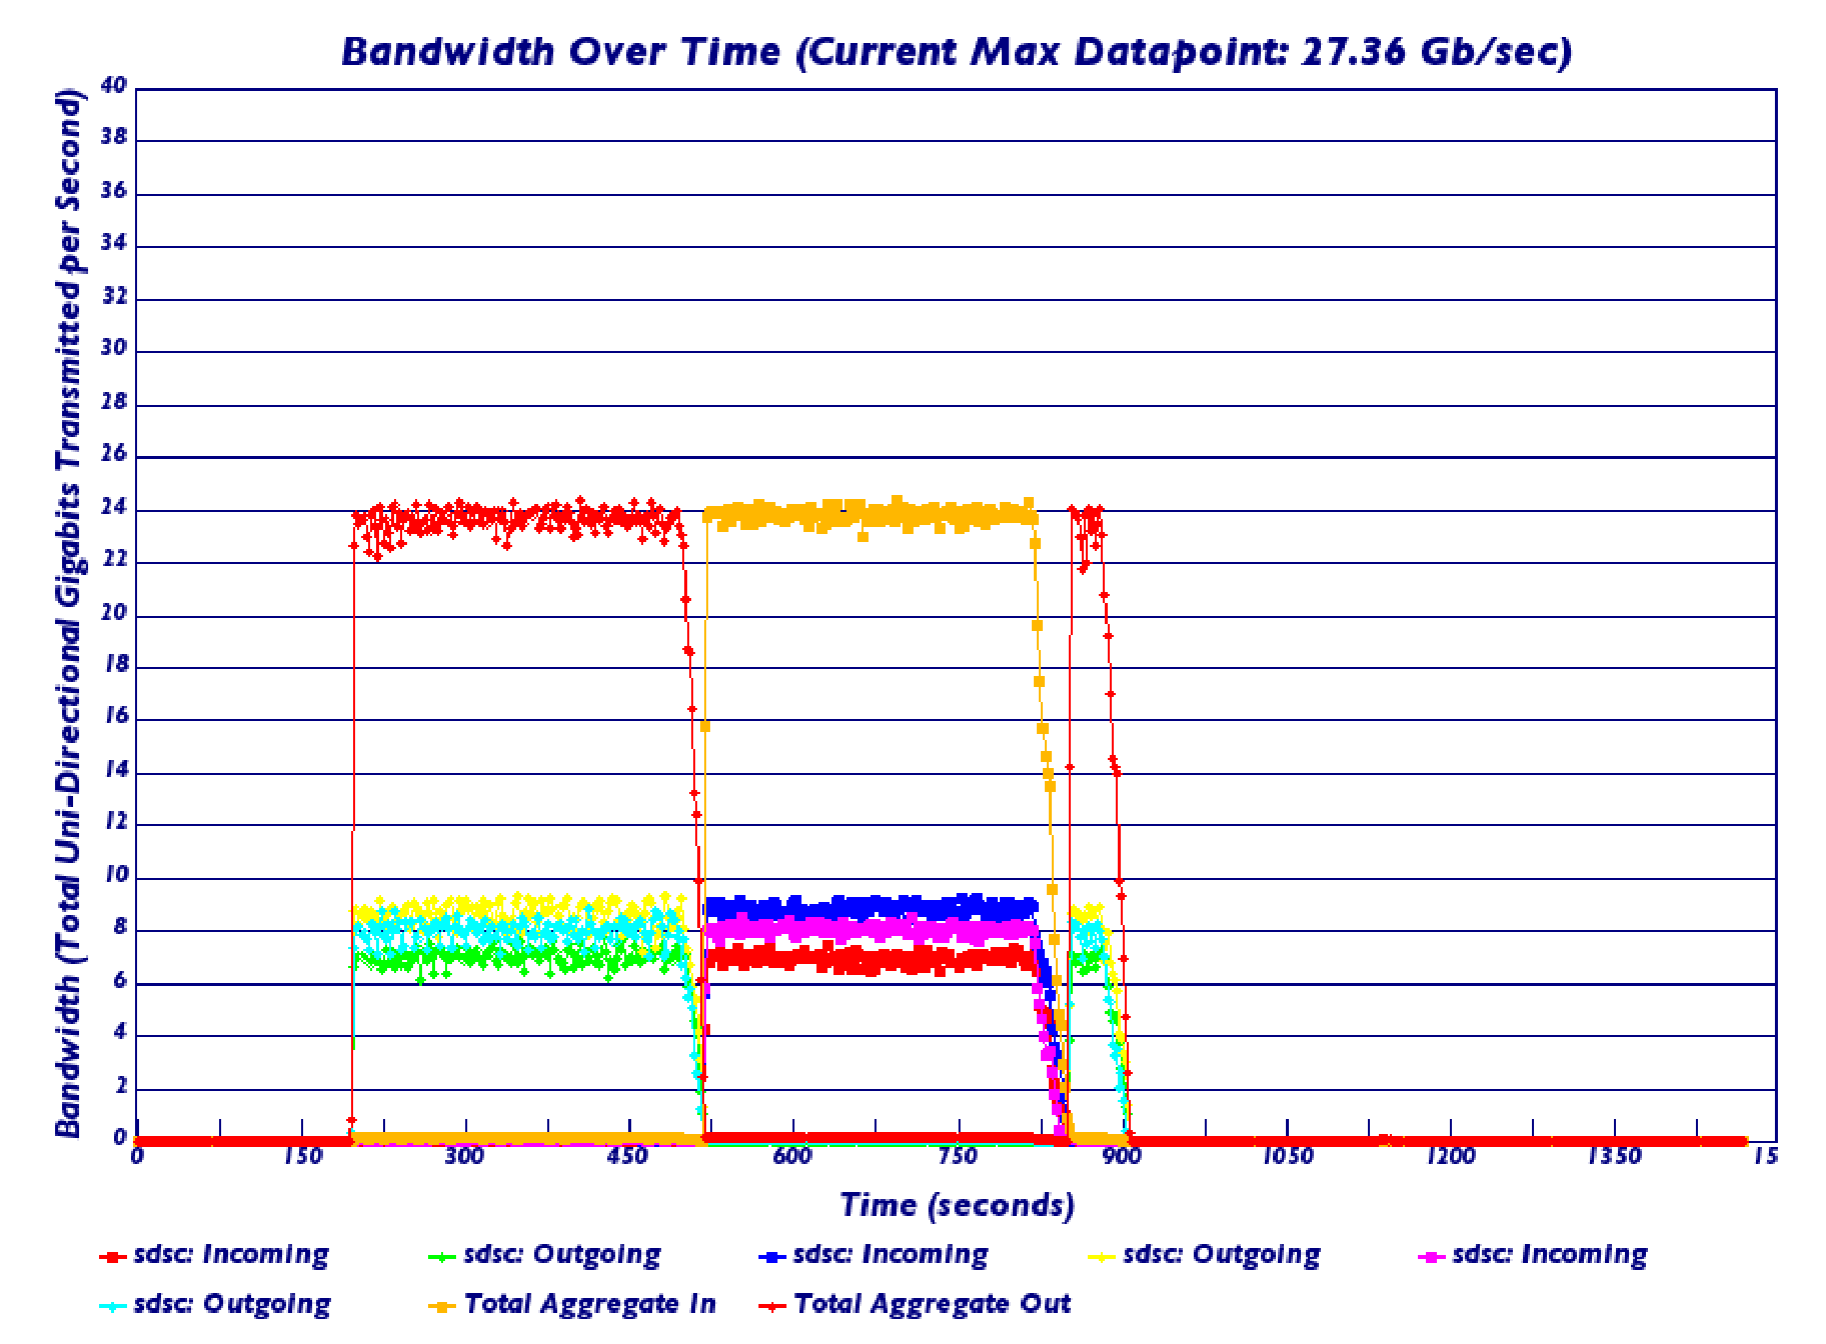
\includegraphics[width=0.99\columnwidth]{image/sc04.png}
\caption{Measured WAN performance at SC'04 for sequential reads and writes.}
\label{fig:sc04}
\end{figure}
%
Andrews et al.~\cite{Andrews2005} have demonstrated the high scalability 
of the GPFS file system in two consecutive SuperComputing (SC) conferences.
%
In these demonstrations, data centers across the US continent are connected
using the GPFS file system.
%
These data centers include: San Diego Supercomputing Center (SDSC) in San
Diego, CA,
the National Center for Supercomputing Applications (NCSA) in 
Urbana, IL, 
and the conference location in Phoenix, AZ and Pittsburgh, PA.
%
In the SC'03 conference, the researchers used a 10Gb/s connection at the 
conference center, and the GPFS achieves around 9Gb/s read/write speed working on 
storage in San Diego.
%
This is about 90\% percent of the connection bandwidth.
%
In the SC'04 conference, the researchers used a 40Gb/s connection at the 
conference center, with GPFS file system connecting to storage in both 
SDSC and NCSA sites.
%
They achieved around 27Gb/s sustaining speed, which is about 67\% of the 
connection bandwidth. 
%
Figure~\ref{fig:sc04} plots the bandwidth overtime in this test.
%
Given the large physical distance (from the west coast to the east coast)
of these experiments, GPFS has demonstrated great scalability.



\subsubsection{GPFS to Achieve Fast Scan}
Distributed file systems are good at providing big throughput, but are traditionally
bad at operations on many small files.
%
Freitas et al.~\cite{freitas2011gpfs} experimented the use of solid state drives
(SSDs) to store the metadata of a file system, and reported satisfactory
result on scanning 10 billion files on a GPFS file system.
%
It took 43 minutes in this test.

The scan over 10 billion files takes 2 steps.
%
In the first step, it parallelly traverses all directories. 
%
Each processor takes care of a sub-tree.
%
When this phase is complete, the full path to every file and that file’s inode number is stored in a series of temporary files.
%
The second step is sequential scan.
%
It begins by assigning the temporary files to the processes running on each node.
%
Each set of temporary files contains a range of inodes in the file system.
%
The files’ inodes are read directly from disk via a GPFS API, thus providing 
the files’ attributes such as owner, file size, atime and it includes 
the files’ extended attributes.
%
Figure~\ref{fig:gpfs_scan} shows the number of reads per second in this test.
%
\begin{figure}
\centering
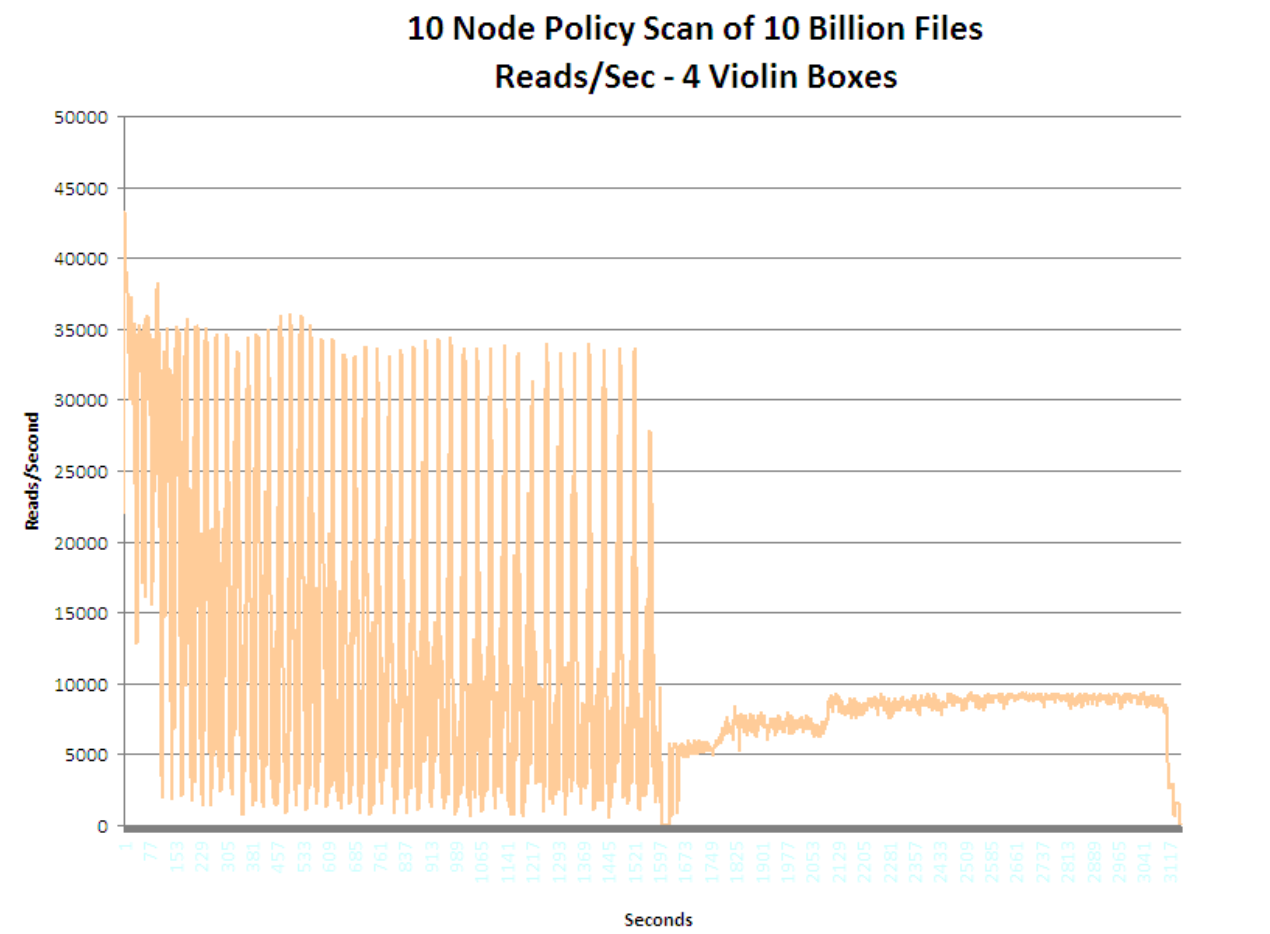
\includegraphics[width=0.99\columnwidth]{image/gpfs_scan.png}
\caption{Aggregate read operations per second.}
\label{fig:gpfs_scan}
\end{figure}

The first step takes about 20 minutes. 
%
This step is highly input operations intensive, because it reads many random
locations in the file system.
%
This step of scan greatly benefits from the underlying SSD storage that keeps 
all the metadata.
%
The second step takes about 23 minutes.
%
It reads the temporary files created by the first phase. 
%
It is essentially bandwidth bound.


\subsubsection{GPFS to Achieve High Bandwidth}
%
\begin{figure}
\centering
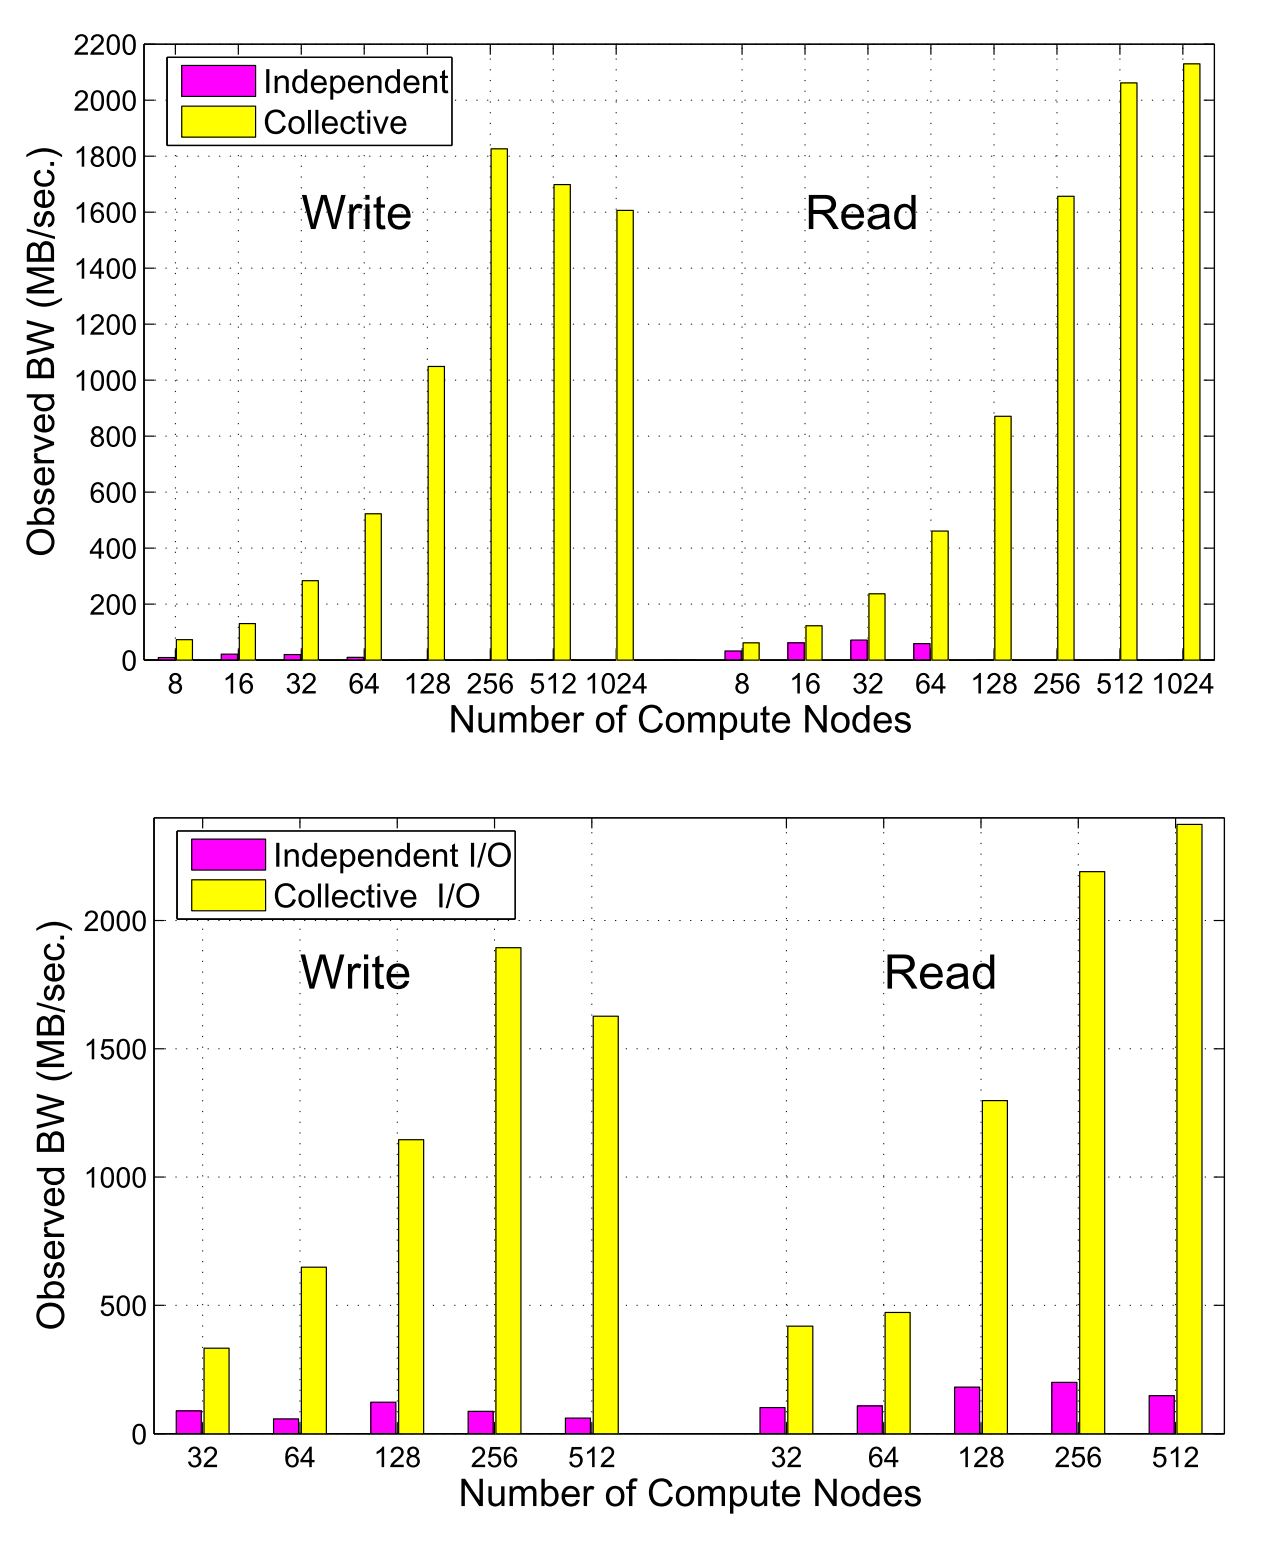
\includegraphics[width=0.99\columnwidth]{image/bw.png}
\caption{Improvement on bandwidth of GPFS file system after applying collective I/O.}
\label{fig:bw}
\end{figure}
%
Ross et al.~\cite{Yu2006} used MPI I/O on top of GPFS to achieve good read/write
performance on an IBM Blue Gene supercomputer.
%
They used the ROMIO MPI implementation, and tuned it to work best with GPFS.
%
For example, they implemented collective buffering in MPI I/O, which 
rearranges and aggregates data in memory prior to writing to files to 
reduce the number of disk accesses.
%
For scientific applications, collective buffering is effective for 
achieving scalable I/O.
%
They also replaced a few MPI implementations based on the characteristics
of the GPFS system.
%
For example, they replaced the use of the point-to-point functions with 
MPI\_Alltoallv, which can utilize up to 98\% of the peak bandwidth within 
a compute node.
%
They also replaced the MPI\_Allgather with an MPI\_Allreduce, 
which performs much better for short and medium sized messages. 
%
The results show that the achieved bandwidth with collective I/O is 
significantly improved, as shown in Figure~\ref{fig:bw}.



\subsection{Higher Performance on Lustre File System}
%
The Lustre file system receives most intensive research because of its
open source nature. 
%
%Here is a selected collection and the main topic of each paper:
For example, Crosby~\cite{Crosby2009} characterized the performance of 
Lustre file system on a real supercomputer system;
%
Xie et al.~\cite{Xie2012} specifically characterized output performance
with respect to a number of system parameters;
%
Schwan~\cite{Schwan2003} and Henschel et al.~\cite{Henschel2012} 
demonstrate implementations of Lustre to achieve the best performance
on real systems; 
%
Lofstead et al.~\cite{lofstead2010managing} specifically researched 
interference effects measured on two real systems; and
%
Shipman et al.~\cite{Shipman2010} summarized real lessons learned 
to achieve high performance on a very large scale Lustre file system.

To focus our discussion on the core performance issues, 
this subsection first identifies a few parameters that affect the performance
of Lustre file system in a real production environment, and then provides
a few demonstrations of Lustre file system to achieve both high scalability
and performance. 


\subsubsection{Performance Characteristics of the Lustre File System}
%
\begin{figure}
\centering
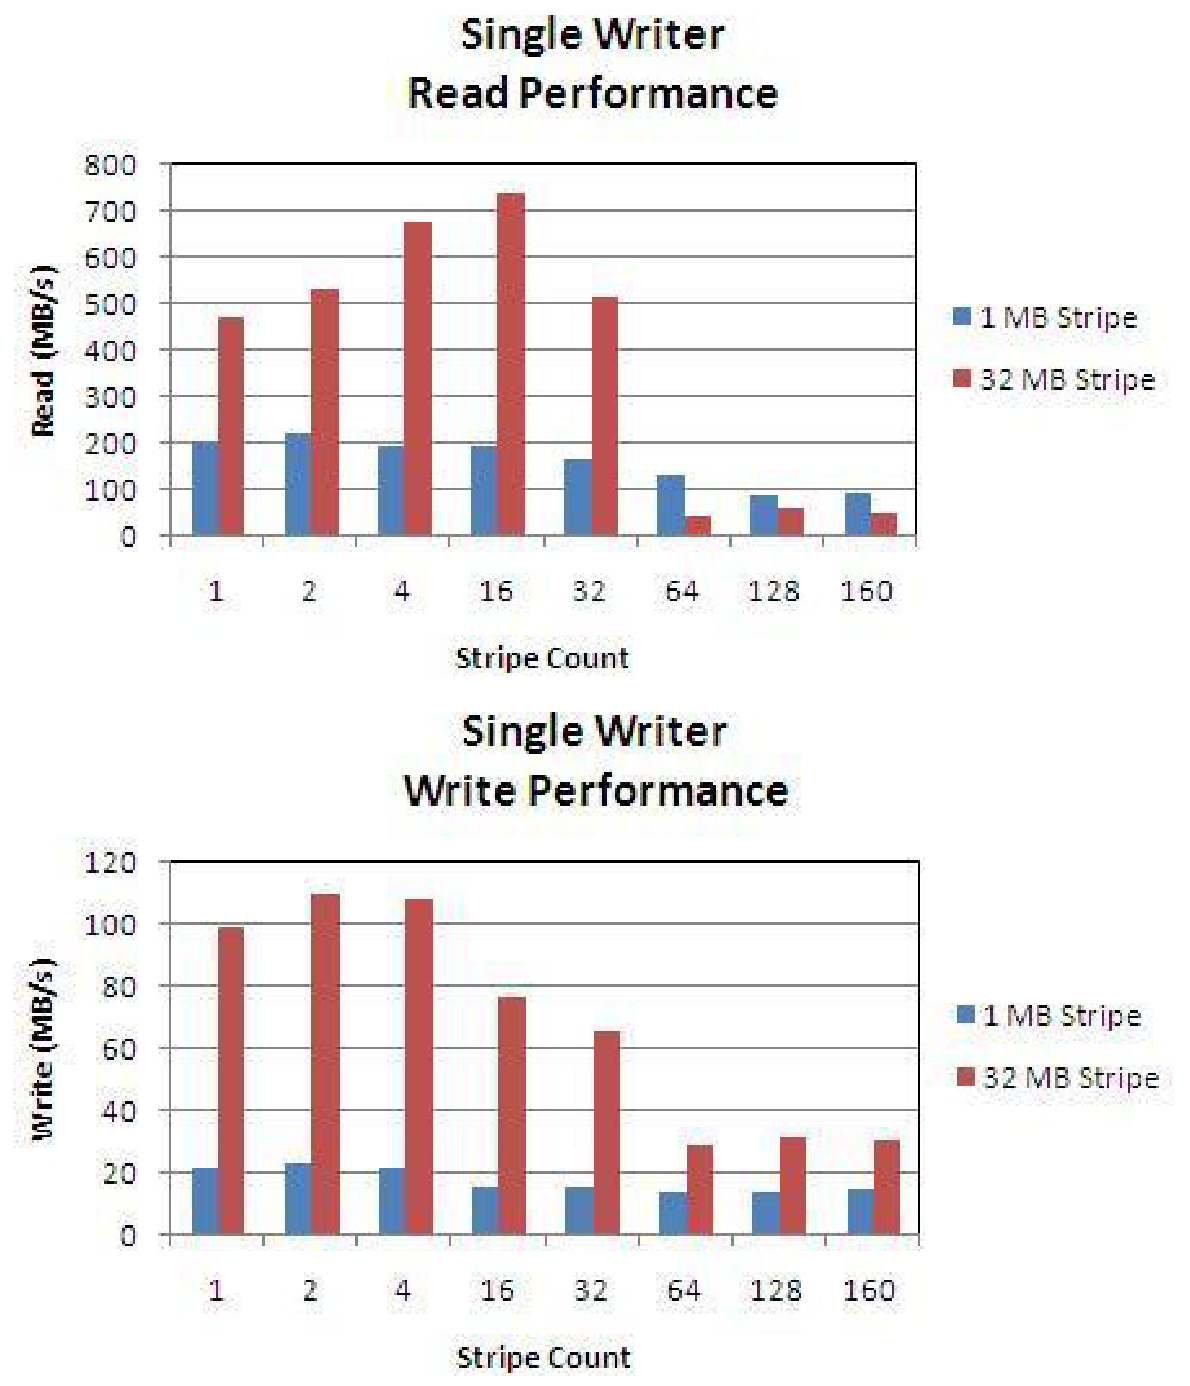
\includegraphics[width=0.99\columnwidth]{image/lustre_rw.png}
\caption{Read and write performance of Luster file system on a real system
	as a function of stripe count.}
\label{fig:lustre_rw}
\end{figure}
%
Crosby et al.~\cite{Crosby2009} characterized the performance of Lustre 
file system on a real system: a Cray XT5 supercomputer at the Oak Ridge
National Lab.
%
Striping is an important mechanism in Lustre to achieve high 
throughput~\ref{sec:stripe_Lustre}, so it is important to test the I/O
performance as a function of the stripe sizes.
%
The researchers performed read and write tests on data files with size
varying from 32MB to 5GB on the real system, and plotted their performance
as shown in Figure~\ref{fig:lustre_rw}.
%
It shows that both write and read performance significantly degrades when
the stripe count is greater than 32, with 16 or 4 probably being the 
sweet spot.
%
These tests also show that a larger sized stripe, for example 32MB other than 
1MB, is helpful to achieve a better performance.


\subsubsection{High Scalability of Luster File System}
%
\begin{figure*}
\centering
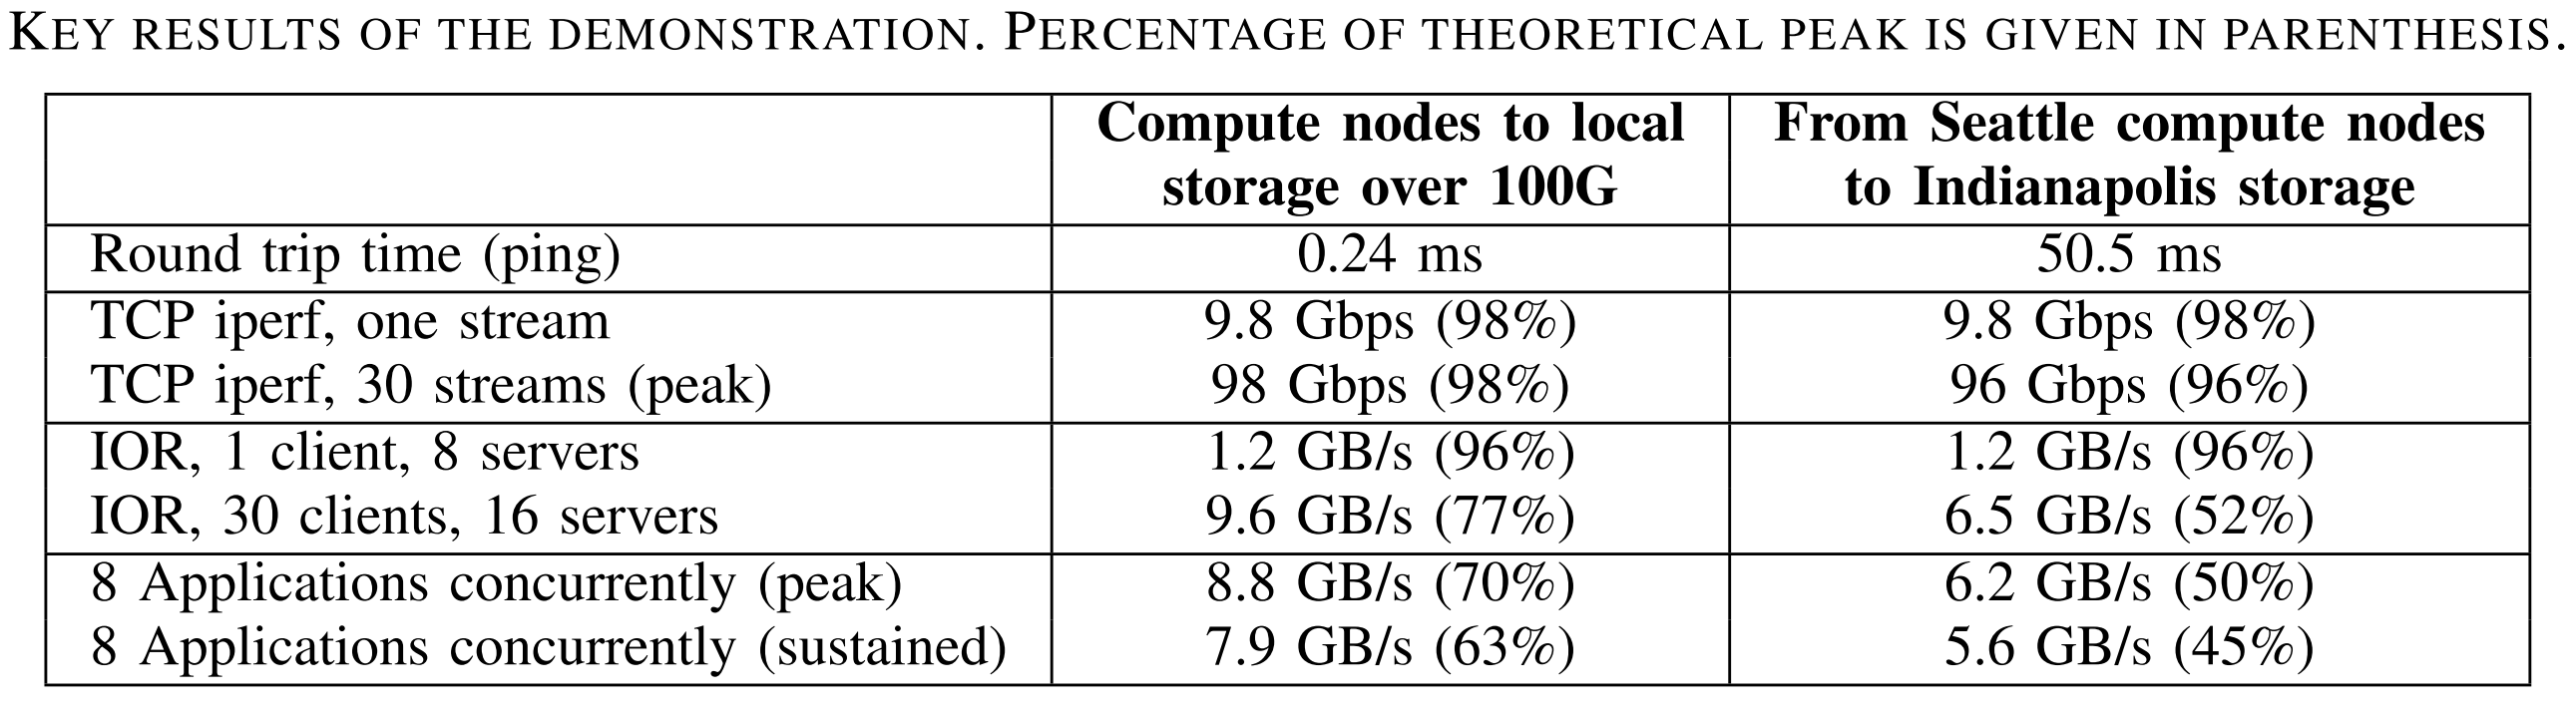
\includegraphics[width=0.9\textwidth]{image/lustre_scale.png}
\caption{Scalability test of Lustre File System. This test compares the same
	software and hardware performing either on the local site, or through a 
	WAN connection.}
\label{fig:lustre_scale}
\end{figure*}
%
Researchers have also investigated the capability of Lustre file system
to achieve a great scalability.
%
Henschel et al.~\cite{Henschel2012} demonstrated a Lustre file system over
a 100Gbps wide area network of 3,500km.
%
These researchers compared the same setups of hardware and software on a local
machine room, as well as spanning from Seattle to Indianapolis.
%
Evaluations are performed on both benchmark test suits as well as real-world
applications.
%
The results are shown in Figure~\ref{fig:lustre_scale}.

These evaluations show a 20\% to 30\% degradation of throughput 
when the file system is set to cross the country.
%
This result is satisfactory considering the many technical difficulties 
associated with a WAN and the complexity of a distributed file system.
%
These results serve as a concept demonstration that a Lustre file system
with very big scales is possible.











